\subsection{\Glsfmtlongpl{rnn} simples}

L'\gls{rnn} le plus simple à imaginer se réduit à une combinaison affine de l'état passé et de l'entrée.
Mathématiquement, une couche d'un tel \gls{rnn} prend la forme suivante
\begin{equation}
    \label{eq.rnn}
    h^{(t)} = \phi\left(Uh^{(t-1)} + Wx^{(t)} + b\right) \qquad 1 \le t \le n
\end{equation}
où \(t\) est le temps\footnote{Il peut être continu ou discret, réel ou abstrait.},
\(x^{(t)}, h^{(t)}\) sont respectivement l'entrée et la sortie à l'instant \(t\), 
\(n\) est la longueur de la séquence et \(\phi\) est la fonction d'activation~\cite{Fathi_2021}.
Dans le cas où \(\phi\) est l'identité,  
la transformée en \(z\) de l'équation~\ref{eq.rnn} est donnée par 
\begin{equation}
    \label{eq.rnn-tz}
    H(z) = z\left(zI - U\right)^{-1} \left(WX(Z) + b\right)
\end{equation}
il s'agit donc d'un système à réponse impulsionnelle infinie~\cite{Fathi_2021}.

Le traitement d'une séquence \(x\) par un \gls{rnn} \(\mathcal{R}\), 
est équivalent à son traitement par un \gls{ffn} \(\mathcal{F}\) dont la profondeur est égale à la longueur de \(x\).
\(\mathcal{F}\) est donc appelé \emph{dépliement temporel} de \(\mathcal{R}\) pour \(x\)
(Voire Figure~\ref{fig.rnn-unfold}).

\begin{figure}[hbt]
    \centering
    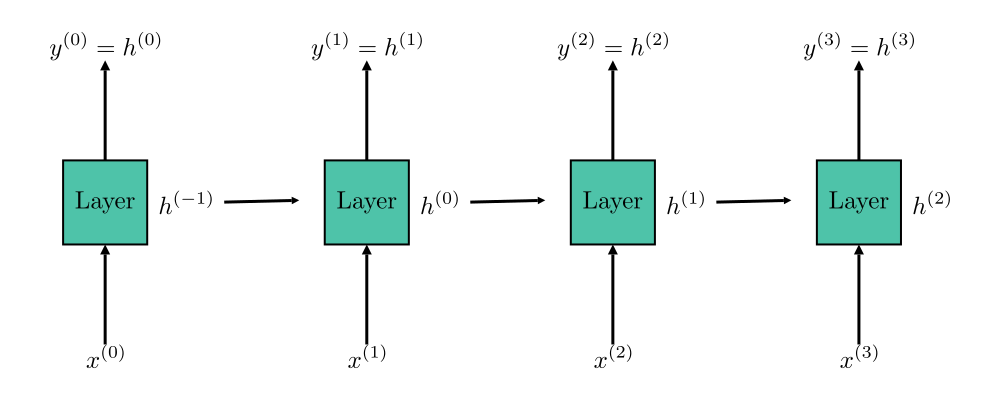
\includegraphics[width=15cm]{rnn-unfolding.png}
    \caption{Dépliement temporel d'un \glsfmtshort{rnn} sur une entrée de longueur 4.}
    \label{fig.rnn-unfold}
\end{figure}


